%Results
\section{Descriptive statistics}

Using the individual weights attributed to each plant, we compute the weighted mean and weighted standard deviation for all variables. Even though we have four variables in our analysis, it is important to notice that there is a high correlation between the variables (see Table \ref{tab:var_correlation}) and that in a future trial, the analysis of other less-correlated variables (non-measured here) could be interesting.\\

\begin{table}[ht]
\rowcolors{2}{gray!25}{white}
\centering
 \caption{Correlation matrix of the four variables.}
\begin{tabular}{lrrrr}
  \toprule
 & DRY\_LS & DRY\_RS & FRESH\_RS & FRESH\_LS \\ 
  \midrule
DRY\_LS & 1.00 & 0.70 & 0.84 & 0.93 \\ 
  DRY\_RS & 0.70 & 1.00 & 0.76 & 0.68 \\ 
  FRESH\_RS & 0.84 & 0.76 & 1.00 & 0.93 \\ 
  FRESH\_LS & 0.93 & 0.68 & 0.93 & 1.00 \\ 
   \bottomrule
\end{tabular}
\label{tab:var_correlation}
\end{table}

Because of germination problems on the platform and inside the germination chamber, not all genotypes were similarly represented in the experiment. Table \ref{tab:updated_germ_rates} presents the effective germination rates for each genotype, i.e. the number of seed actually kept for the spatial analysis over the number of seeds placed on the platform. This table is interesting because germination rate is a genotypic feature. We see clear discrepancies between genotypes, some have high germination rates (e.g. genotypes 29 and 22 both havee germination rate higher than 90\%) while 6 genotypes have a germination rate lower than 50\% (below the dashed line on Table \ref{tab:updated_germ_rates}), even though more than 15 seeds per genotype were placed on the platform. This indicates that all the genotypes, used in this experiment, may not be well suited to aeroponic growth.\\

\begin{table}[hbtp]
  \rowcolors{2}{gray!25}{white}
\centering
\caption[Effective germination rates]{Effective on-platform germination rates (GR) with the number of seeds kept for data analysis (NS kept) and the number 
of seeds actually placed on the platform (NS placed) for each genotype. The dotted line represents the 50\% germination rate limit.} 
\begin{minipage}{0.45\textwidth}
\begin{tabular}{lrrr}
  \toprule
Genotype & NS placed & NS kept & GR \\ 
  \midrule
25 & 29 & 27 & 93.1 \\ 
  23 & 22 & 20 & 90.9 \\ 
  16 & 27 & 23 & 85.2 \\ 
  18 & 26 & 22 & 84.6 \\ 
  3 & 29 & 24 & 82.8 \\ 
  17 & 27 & 21 & 77.8 \\ 
  19 & 30 & 23 & 76.7 \\ 
  1 & 24 & 18 & 75.0 \\ 
  12 & 28 & 21 & 75.0 \\ 
  14 & 26 & 19 & 73.1 \\ 
  28 & 26 & 19 & 73.1 \\ 
  9 & 29 & 20 & 69.0 \\ 
  6 & 29 & 19 & 65.5 \\ 
  7 & 29 & 19 & 65.5 \\ 
  4 & 23 & 15 & 65.2 \\
  \vdots & \vdots & \vdots & \vdots \\
  \bottomrule
 \end{tabular}
 
\end{minipage} \hfill
\begin{minipage}{0.45\textwidth}
 \begin{tabular}{lrrr}
   \toprule
Genotype & NS placed & NS kept & GR \\ 
  \midrule
    \vdots & \vdots & \vdots & \vdots \\
  27 & 29 & 18 & 62.1 \\ 
  21 & 26 & 16 & 61.5 \\ 
  5 & 30 & 18 & 60.0 \\ 
  24 & 30 & 18 & 60.0 \\ 
  10 & 29 & 17 & 58.6 \\ 
  20 & 26 & 15 & 57.7 \\ 
  22 & 18 & 10 & 55.6 \\ 
  29 & 28 & 15 & 53.6 \\ 
  13 & 27 & 14 & 51.9 \\\hdashline 
  15 & 18 & 9 & 50.0 \\ 
  2 & 26 & 12 & 46.2 \\ 
  11 & 19 & 8 & 42.1 \\ 
  26 & 29 & 12 & 41.4 \\ 
  8 & 21 & 8 & 38.1 \\ 
  30 & 23 & 3 & 13.0 \\ 
   \bottomrule
\end{tabular}

 \end{minipage}
\label{tab:updated_germ_rates}
\end{table}

Using the weighted means and standard deviations, we created boxplots ordered by descending mean value for tank A, presented in Figure \ref{fig:dotplot_all_variables}. The numerical values of these results are presented in Table \ref{tab:summary_table_all_variables}, in Appendix \ref{appendix:mean_std_table}.
It is clear that values for tank A are almost always higher than for tank B expect for some genotypes (e.g. genotype 12 on all variables and genotype 11 on the dry weights), even if there seems to be more variation in tank A. A t-test proved this difference to be highly significant\footnote{The test were performed with a significance level, $\alpha$ = 0.05.} (see Table \ref{tab:mean_diff_between_tanks_t_test}). However, the value for tank B is higher for some genotypes (e.g. genotype 12 for all variables and genotype 11 for the dry weights). This shows that those genotypes might be more suited to a still growing environment.\\

\begin{table}[hbtp]
  \rowcolors{2}{gray!25}{white}
\centering
\caption[Mean difference between the 2 tanks]{Mean weight value (g) for each tank with associated p-value from a t-test for the difference of means between the two tanks}
\begin{tabular}{lrrrr}
  \toprule
 & FRESH\_LS & FRESH\_RS & DRY\_LS & DRY\_RS \\ 
  \midrule
Mean value in tank A  & 2.604 & 3.09 & 0.1963 & 0.1964 \\ 
Mean value in tank B & 1.755 & 1.79 & 0.1725 & 0.1666 \\ 
  p-value & $<$0.001 & $<$0.001 & 0.003 & $<$0.001 \\ 
   \bottomrule
\end{tabular}
\label{tab:mean_diff_between_tanks_t_test}
\end{table}

To further assess difference in means between the two tanks, we performed a paired t-test of the means difference between the two tanks, for all variables. The resulting p-values are presented in table \ref{tab:ind_geno_t_test_pval} in Appendix \ref{appendix:t_test}. We see that the difference in mainly significant for the fresh weights (which is also visible on Figure \ref{fig:dotplot_all_variables} \textbf{a} and \textbf{b}) and only for a handful of genotypes (6, 23, 10, 26, 4 and 8). We chose to use multiple univariate t-tests, because multivariate t-tests are extremely sensitive. Any violation to the multivariate normality assumption and equality of variance-covariance matrices will lead a significant result.

\begin{figure}
\centering
	\begin{subfigure}[t]{\textwidth}
	\label{fig:desc_stat_DRY_LS}
		\centering
		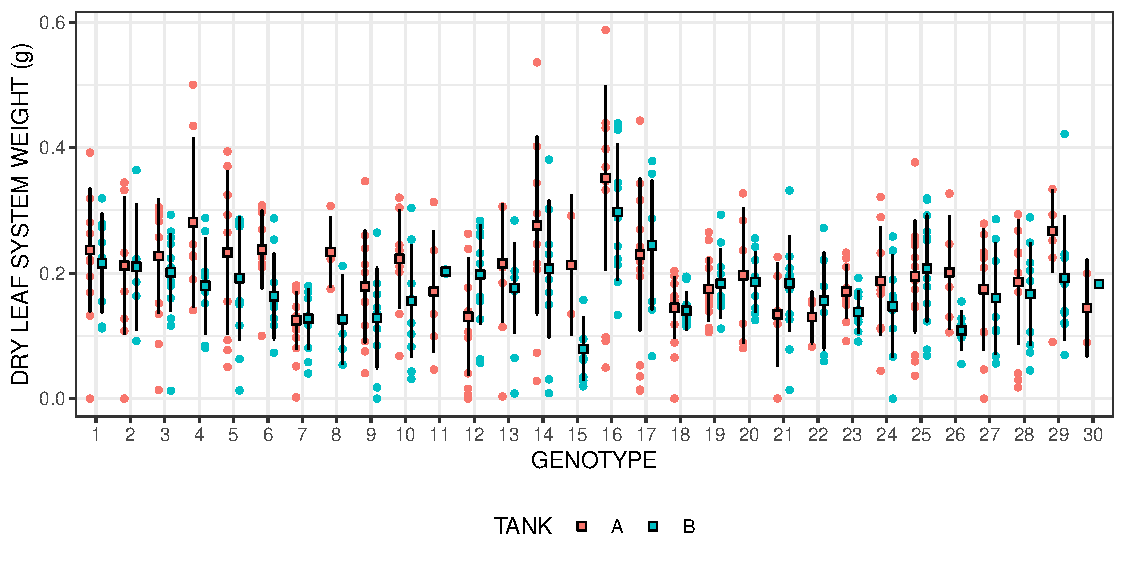
\includegraphics[width = \textwidth]{../../Figures/DRY_LS_summary_plot.pdf}
		\caption{Dry leaf weight ($DRY\_LS$)}
			\end{subfigure}

	\begin{subfigure}[t]{\textwidth}
		\centering
		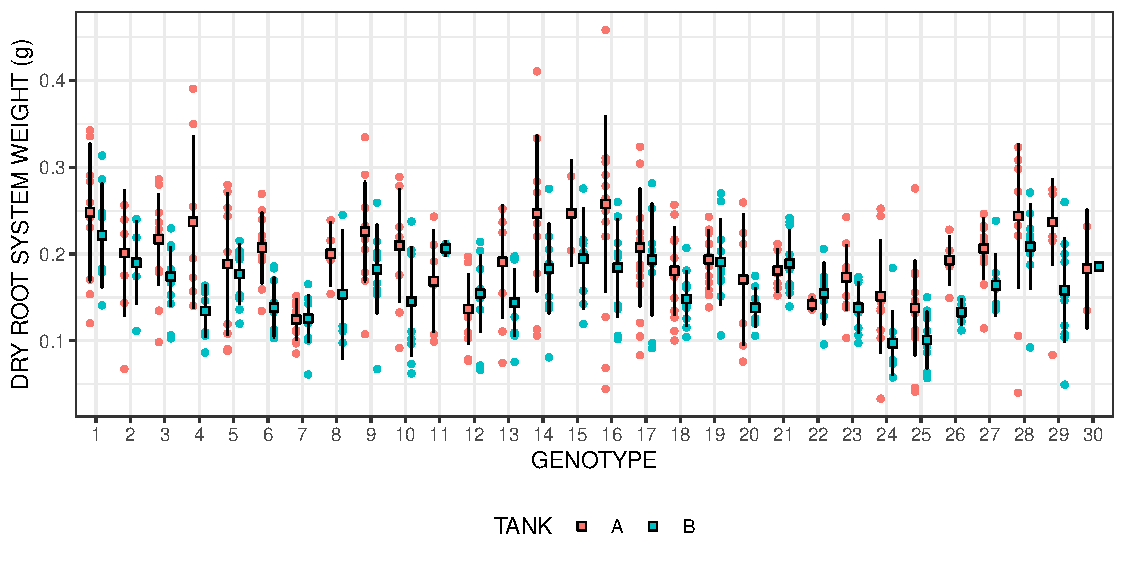
\includegraphics[width = \textwidth]{../../Figures/DRY_RS_summary_plot.pdf}
		\caption{Dry root weight ($DRY\_RS$)}
	\end{subfigure}
	\caption[Boxplot of the mean weight and associated standard deviation]{Boxplot displaying mean weight (\protect\emptysquare) and associated standard deviation (\protect\blackline), grouped by tanks and ordered by descending mean value for tank A.}
\end{figure}
\begin{figure}\ContinuedFloat
	\captionsetup[figure]{list=no}
	\begin{subfigure}[t]{\textwidth}
		\centering
		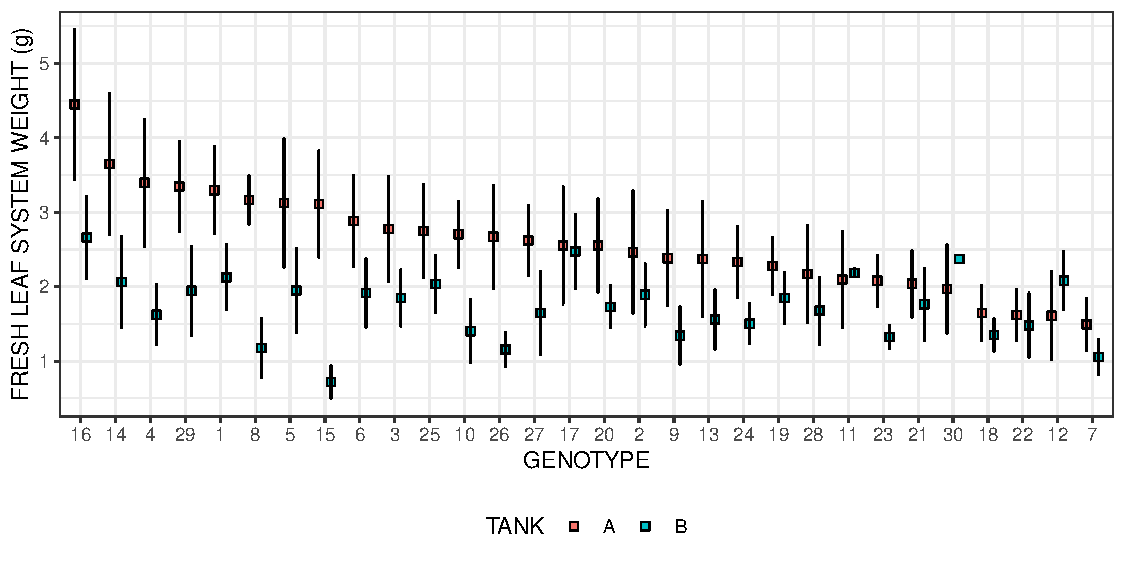
\includegraphics[width = \textwidth]{../../Figures/FRESH_LS_summary_plot.pdf}
		\caption{Fresh leaf weight ($FRESH\_LS$)}
	\end{subfigure}

	\begin{subfigure}[t]{\textwidth}
		\centering
		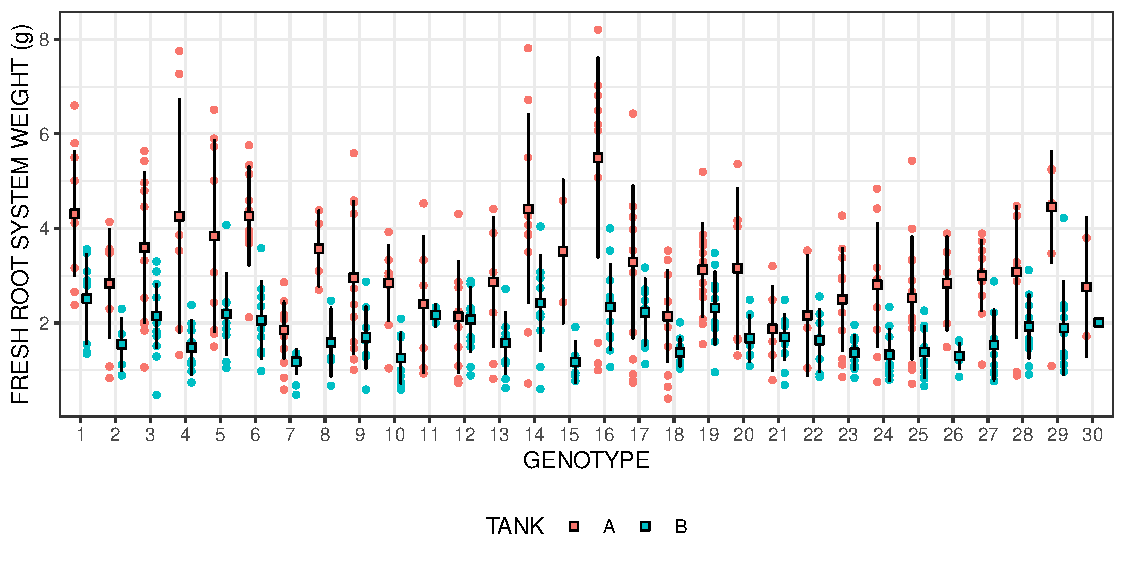
\includegraphics[width = \textwidth]{../../Figures/FRESH_RS_summary_plot.pdf}
		\caption{Fresh root weight ($FRESH\_RS$)}
	\end{subfigure}
	\caption[Boxplot of the mean weight and associated standard deviation]{Boxplot displaying mean weight (\protect\emptysquare) and associated standard deviation (\protect\blackline), grouped by tanks and order by descending mean value for tank A.}
	\label{fig:dotplot_all_variables}
\end{figure}

\section{SpATS analysis}
For the SpATS model, we analysed the four weight variables using the following model:
\begin{equation}
	\mathbf{y} =\mathbf{X} \boldsymbol{\beta}_{T} +\mathbf{X}_{s} \boldsymbol{\beta}_{s}+\mathbf{Z}_{s} \boldsymbol{s}+\mathbf{Z}_{u} \boldsymbol{u}
	+ \mathbf{Z}_{v} \boldsymbol{v} + \mathbf{Z}_{g} \boldsymbol{g}+ \boldsymbol{\varepsilon} \text{,}
\end{equation}
where:
\begin{itemize}
	\item $\mathbf{X} \beta_{T}$ is the fixed term for the tanks,
	\item $\mathbf{X}_{s} \boldsymbol{\beta}_{s}+\mathbf{Z}_{s} \boldsymbol{s}$ is the mixed model representation of the bivariate smooth surface $f(\boldsymbol{u},\boldsymbol{v})$,
	\item $\mathbf{Z}_{u} \boldsymbol{u}$ is the random effect of the rows,
	\item $\mathbf{Z}_{v} \boldsymbol{v}$ is the random effect for the columns,
	\item $\mathbf{Z}_{g} \boldsymbol{g}$ is the random effect for the genotypes, and 
	\item $\boldsymbol{\varepsilon}$ is the residual error.
\end{itemize}

The analysis of the results is split in 2 parts:
\begin{enumerate}
	\item A visual analysis of the fitted values and the residuals compared to the raw data; to see if the 
	spatial patterns have been accounted for by the spatial model.
	\item An analysis of the individual contribution of each term of the bivariate smooth surface $f(\boldsymbol{u},\boldsymbol{v})$, using the effective dimensions.
	%\item A comparison of the variance of all the random term to see which one were the most influential in the model.
\end{enumerate}
The analysis of the estimated coefficient for the genotypes and for the tanks is presented in a following section, with the estimates of the BSS model.

\subsection{Visual analysis}
The raw data, the fitted data and the spatial model residuals are presented, for all variables, in Figure \ref{fig:spats_model_results}. The difference between tanks is more pronounced for the fresh weights than for the dry weights, just as stated in the previous section. However, this difference is well represented in the fitted data, where tank B (on the right in each picture) consistently display lower weight values. A strip effect is also noticeable for tank B, where the last strips have lower values than the first ones. This might be an effect of the still growing environment, since this effect is not present in tank A, which was constantly moving.\\

No clear pattern emerges from the residuals, expect the fact that tank A seems to have more single data point with lower values that were not picked up by the spatial surface. This means that tank A had more local heterogeneities. Indeed, when we consider the movement in tank A, it makes sense not to see clear spatial trends revealed in the data, and rather having a wider variations among the residuals. A analysis of the residuals distribution revealed no violation to the normality assumption.\\

Furthermore, a comparison of the scales of the fitted values and the raw data on Figure \ref{fig:spats_model_results} shows us that the smooth surface could not account for the extreme values present in the raw data. For example the scale of the weight values for FRESH\_RS goes from 0 to 8, whereas it only goes from 0 to to 5 for the fitted surface. However, the scale of the residuals is lower than the one of the fitted values, indicating that the smooth surface accounts for a good amount of the spatial variation.

\begin{figure}
	\begin{subfigure}[t]{\textwidth}
		\centering
		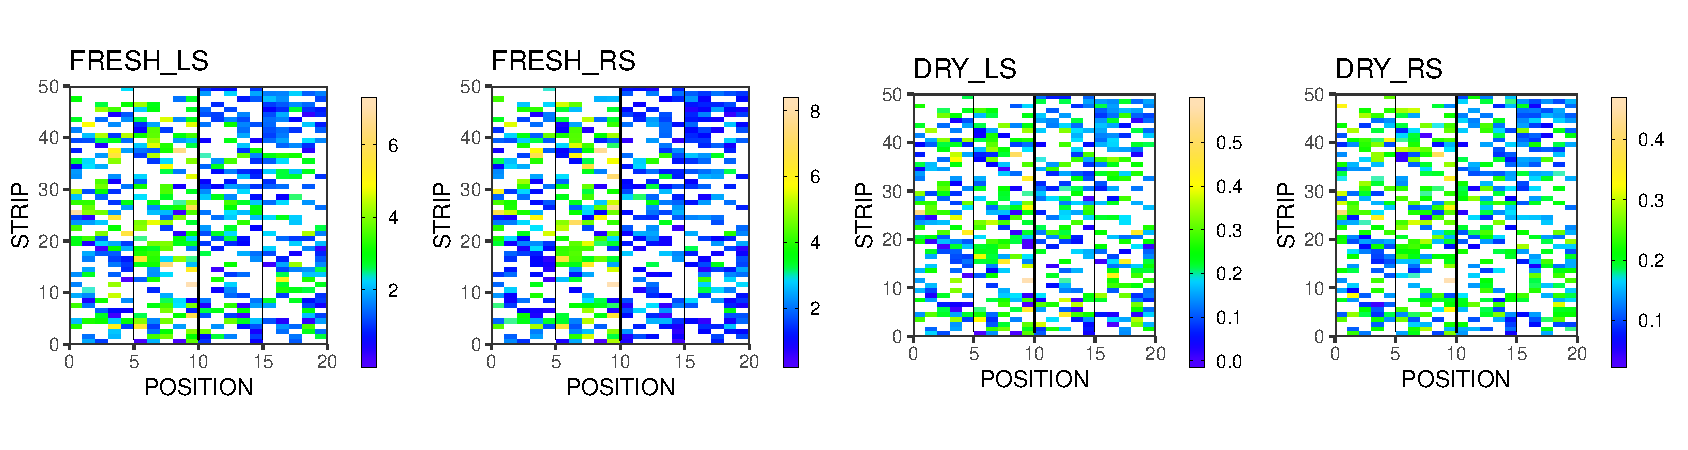
\includegraphics[width = \textwidth]{../../Figures/SPATS_rawData_plot.pdf}
		\caption{Raw data}
	\end{subfigure}
	
	\begin{subfigure}[t]{\textwidth}
		\centering
		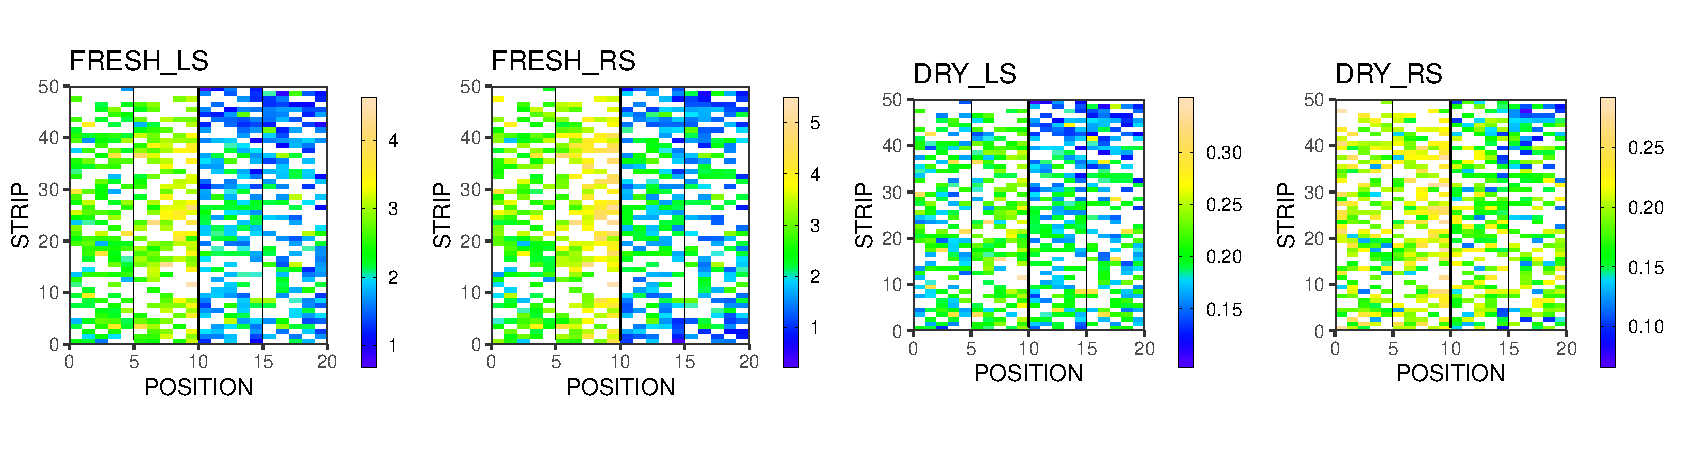
\includegraphics[width = \textwidth]{../../Figures/SPATS_Fitted_plot.pdf}
		\caption{Fitted spatial trend}
	\end{subfigure}
	
	\begin{subfigure}[t]{\textwidth}
		\centering
		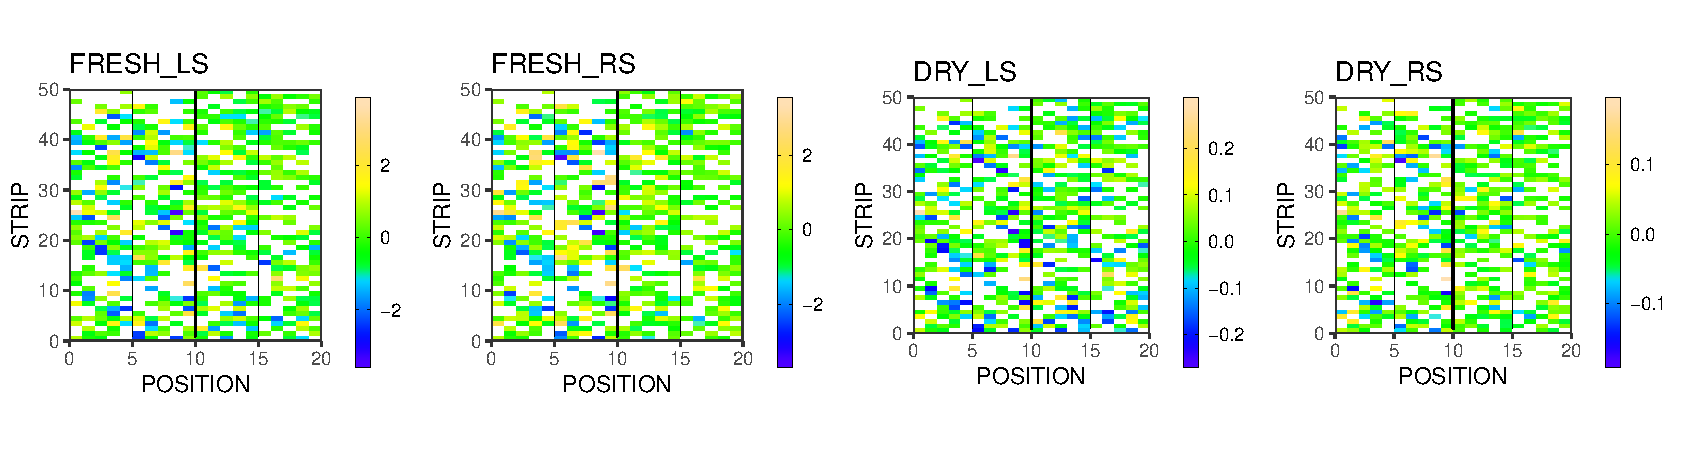
\includegraphics[width = \textwidth]{../../Figures/SPATS_residuals_plot.pdf}
		\caption{Residuals' spatial plot}
	\end{subfigure}
	\caption{Raw data, fitted spatial trend and residuals' plot for each variable.}
	\label{fig:spats_model_results}
\end{figure}

\subsection{Smooth surface terms analysis}
The smooth part of the smooth bivariate surface can be decomposed in the following terms:
\begin{equation}
	f(\boldsymbol{u},\boldsymbol{v}) = f_{u}(\boldsymbol{u})+f_{v}(\boldsymbol{v})+\boldsymbol{u} \odot h_{v}(\boldsymbol{v})+\boldsymbol{v} \odot h_{u}(\boldsymbol{u})+f_{u, v}(\boldsymbol{u}, \boldsymbol{v}) \text{,}
\end{equation}
that are linear terms, linear-by smooth and smooth-by-smooth interaction terms (see section \ref{sec:spats_model} for more details). The contribution of each term to the whole surface can be assessed using the effective dimension of each component. Table \ref{tab:spats_dimensions} presents the contribution of each term for each variable as the percentage of the total effective dimension of the smooth surface.\\

For the fresh weights, the smooth-by-smooth interaction ($f_{u, v}(\boldsymbol{u}, \boldsymbol{v})$) represents almost 70\% of the total surface variation. This emphasizes the complexity of the spatial patterns. The smooth-by-linear along the strips interaction ($\boldsymbol{u} \odot h_{v}(\boldsymbol{v})$) and the smooth along the strips ($f_{u}(\mathbf{u})$ ) terms account for the rest of the variation. This confirms that there is more variation along the strips than along the positions.\\

For the dry weights, the variation is shared among all the terms except for smooth along the position that accounts for nothing. This means that there were less heterogeneous spatial variation and more smooth gradients than for the fresh weights. Indeed, if we look back at the fitted residuals on Figure \ref{fig:spats_model_results}, we see clearly that there is a gradient among the strips and the positions, instead of random patches of high yield.\\

The total effective dimension is also displayed in the table, because it is an indicator of the overall complexity of the spatial patterns that the smooth surface models. Since the total is lower for the dry weights, it confirms again that the spatial variability was less complex for those variables. As explained in the previous chapter, the effective dimension of a parameter, is proportional to its variance. Therefore, a table presenting the variance of all the random components of the models is presented in Appendix \ref{appendix:tab_spats_variances}

% Table generated by Excel2LaTeX from sheet 'Sheet2'
\begin{table}[htbp]
  \rowcolors{2}{gray!25}{white}
  \centering
  \caption[Effective dimensions of the SpATS model]{Contribution of each component of the spatial smooth surface as a percentage 
  of the total effective dimension of the surface. Here $\boldsymbol{v}$ represents the columns, i.e. the position on the strip; 
  and $\boldsymbol{u}$ represents the rows, i.e. the strip itself.}
	\begin{threeparttable}  
  	    \begin{tabular}{lrrrr}
	    \toprule
	    \begin{tabular}[b]{@{}l@{}}Model \\ \rowcolor{white} components\end{tabular} & \multicolumn{1}{l}{FRESH\_LS} & 
	    \multicolumn{1}{l}{FRESH\_RS} & \multicolumn{1}{l}{DRY\_LS} & \multicolumn{1}{l}{DRY\_RS} \\
	    \midrule
	    $f_{v}(\mathbf{v})$ 								& 0\tnote{$\dagger$} & 0 & 0 & 0  \\
	    $f_{u}(\mathbf{u})$ 								& 8.73 & 14,10 & 17,26 & 17,26 \\
	    $\boldsymbol{u} \odot h_{v}(\boldsymbol{v})$ 		& 19,95 & 16,40 & 24,77 & 24,77 \\
	    $\boldsymbol{v} \odot h_{u}(\boldsymbol{u})$ 		& 2,56 & 0 & 18,36 & 18,36 \\
	    $f_{u, v}(\boldsymbol{u}, \boldsymbol{v})$ 			& 68,76 & 69,5 & 39,62 & 39,62 \\
	    \midrule
	    Total 												& 9,21 (100\%) & 16,15 (100\%) & 5,93 (100\%)& 4,91 (100\%) \\
	    \bottomrule
	    \end{tabular}%
	    \begin{tablenotes}
	    	\item[$\dagger$] All values inferior to 0.0001\% were marked as 0 in the table.
	  	\end{tablenotes}
	\end{threeparttable}
  \label{tab:spats_dimensions}%
\end{table}%


\section{Standard spatial model analysis}
For the standard spatial model analysis,we fitted a baseline model, only considering a fixed effect for the tanks and a random effect for the genotypes and spatially independent residuals:
\begin{equation}
	\mathbf{y} =\mathbf{X} \boldsymbol{\beta}_{T} + \mathbf{Z}_{g} \mathbf{g}+ \mathbf{e} \text{.}
\end{equation}
The model was then augmented separately for each variable, by adding linear regression terms on the rows and columns and one of the following covariance structure:
\begin{itemize}
\item $AR(1)$ process along the rows or columns
\item $AR(1) \times AR(1)$ process
\item $LV$ process along the rows or columns
\item Superimposed row and column structure $LV + LV$
\item Separable process along the rows or columns $LV\otimes J$
\item Separable process along the rows and columns $LV \times LV$
\end{itemize}
At each step, the AIC  was computed and used to select the best model (a lower value is preferred). Table \ref{tab:selected_BSS_models} gives the structure of the final selected model for each variable.\\

\begin{table}[htbp]
  \rowcolors{2}{gray!25}{white}
  \centering
  \caption[Selected BSS models]{Best standard spatial (BSS) model selected for each of the four variables. All the models 
  contain an intercept and a fixed effect for the tank and a random effect for the genotypes. $P$ represents a random effect for the positions (columns), $S$ a random effect for the strips (rows) and $n$ represent the spatially independent residuals.}
    \begin{tabular}{ll}
    \toprule
    Variable & \multicolumn{1}{l}{BSS} \\
    \midrule
    FRESH\_LS & $ S + AR(1) \times AR(1)$  \\
    FRESH\_RS &  $ S + AR(1) \times AR(1)$ \\
    DRY\_LS & $S + P + LV\times LV$ \\
    DRY\_RS &  $S + P + LV+LV$\\
    \bottomrule
    \end{tabular}%
\label{tab:selected_BSS_models}
\end{table}%

First, we see that, for the fresh weights, the models only contains a random effect on the strips (rows) and not the positions (columns). This is similar to the interpretation of the effective dimensions of the SpATS model from Table \ref{tab:spats_dimensions}, that highlighted the strong strip effect and the almost non-existing position effect for the fresh weights. However, all models used a strips-by-positions covariance structure, illustrating the fact that the spatial trends display complex patterns that cannot be accounted for by a one dimensional process only. \\

Then, we see that the fresh weights were best represented by an auto-regressive process whereas the dry weights needed a linear covariance structure. \textcite{piepho_linear_2010} explain that both structures give similar results with large auto-correlation ($\rho$) values, which is the case here (see table \ref{tab:BSS_variance_values}) but that the LV structure is more robust to convergence issues. Since we encountered some convergence problems when fitting the $AR(1)$ structure on the dry weight models, it might explain the better AIC value of the $LV$ models.\\

Finally, both dry weight models use a linear covariance structure but DRY\_LS uses the superimposed structures whereas DRY\_LS uses the separable model. The only difference between those models is the way they model the pairwise variances for plots on different strips (rows) and different positions (columns), but it is not relevant here, as they yield similar results in most cases \parencite{piepho_linear_2010}.\\

Table \ref{tab:BSS_variance_values} presents the auto-correlation values for the two fresh weight models (since the dry weights models do not use an auto-regressive covariance structure). We see that both models exhibit high auto-correlation, however, it is slightly less pronounced over the positions than over the strips. These high values mean that there is a high spatial variation for both variables, which is similar to the conclusions from the SpATS model. However, \textcite{piepho_problems_2015} suggest that auto-correlation values close to one indicates confounding between the trends and the rows/strips. This might explain the absence of a random term for position in the BSS models for the fresh weights (Table \ref{tab:selected_BSS_models}).

\begin{table}[htbp]
\rowcolors{2}{gray!25}{white}
  \centering
  \caption[Auto-correlation values for the BSS models]{Auto-correlation values along the strips ($\rho_{s}$) and the positions ($\rho_{p}$), for the two BSS models using an $AR(1) \times AR(1)$ spatial covariance structure.}
    \begin{tabular}{lrr}
    \toprule
    Variable & \multicolumn{1}{l}{$\rho_{s}$} & \multicolumn{1}{l}{$\rho_{p}$} \\
    \midrule
    FRESH\_LS &   0,998    &    0,992 \\
    FRESH\_RS &   0,993    &   0,952  \\
    \bottomrule
    \end{tabular}%
  \label{tab:BSS_variance_values}%
\end{table}%

\subsection{Visual analysis}
Figure \ref{fig:BSS_model_results} presents the raw data, the fitted values and the residuals of each variables, in a similar fashion than for the SpATS model. We see that the fitted data are very similar to those of the SpATS model and capture the spatial trends correctly. Furthermore, the range of the residuals is similar to the SpATS model, meaning that there are no visual clues indicating that the BSS model is better or worse than the SpATS model.

\begin{figure}
	\begin{subfigure}[t]{\textwidth}
		\centering
		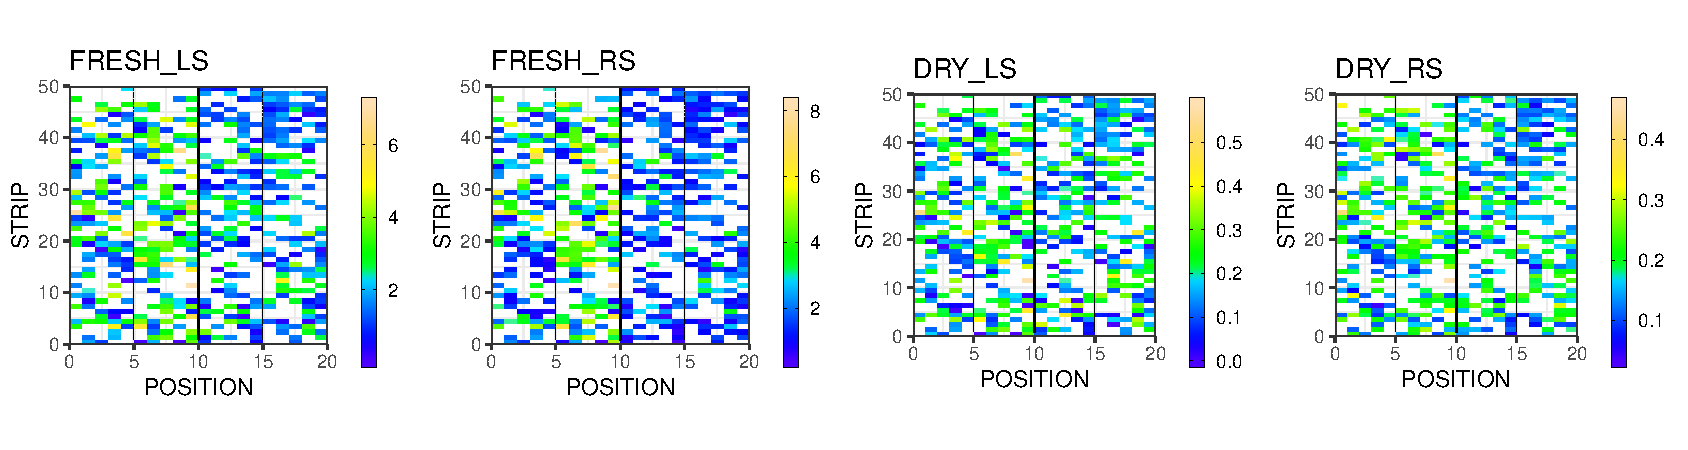
\includegraphics[width = \textwidth]{../../Figures/BSS_rawData_plot.pdf}
		\caption{Raw data}
	\end{subfigure}
	
	\begin{subfigure}[t]{\textwidth}
		\centering
		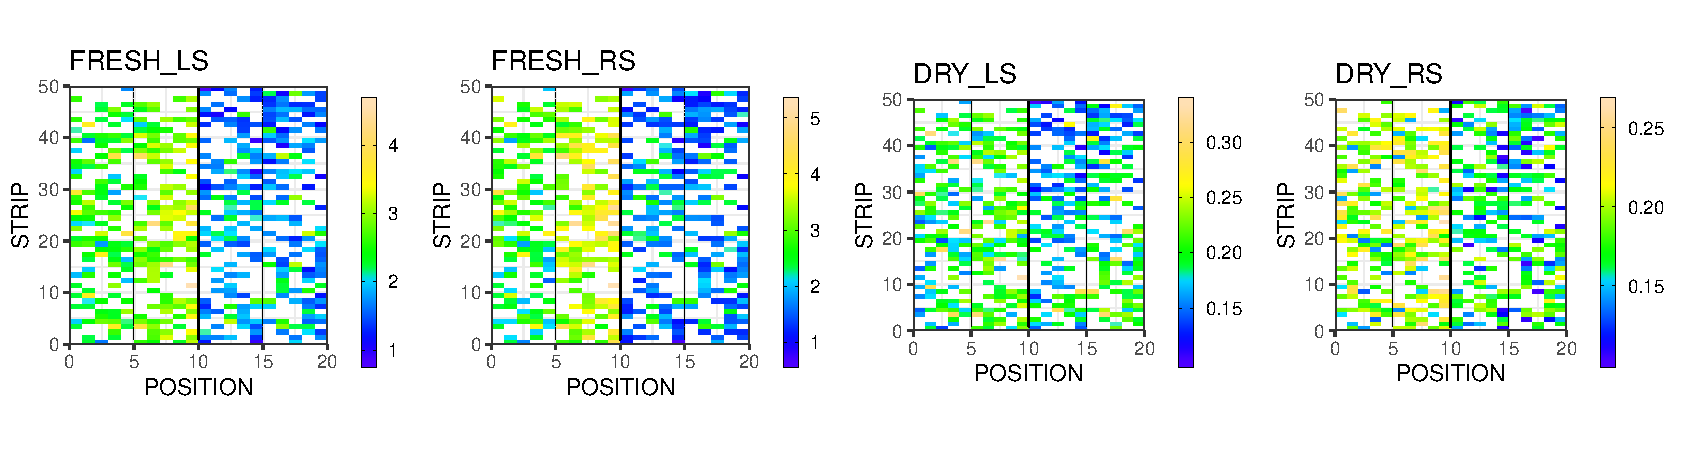
\includegraphics[width = \textwidth]{../../Figures/BSS_FittedData_plot.pdf}
		\caption{Fitted spatial trend}
	\end{subfigure}
	
	\begin{subfigure}[t]{\textwidth}
		\centering
		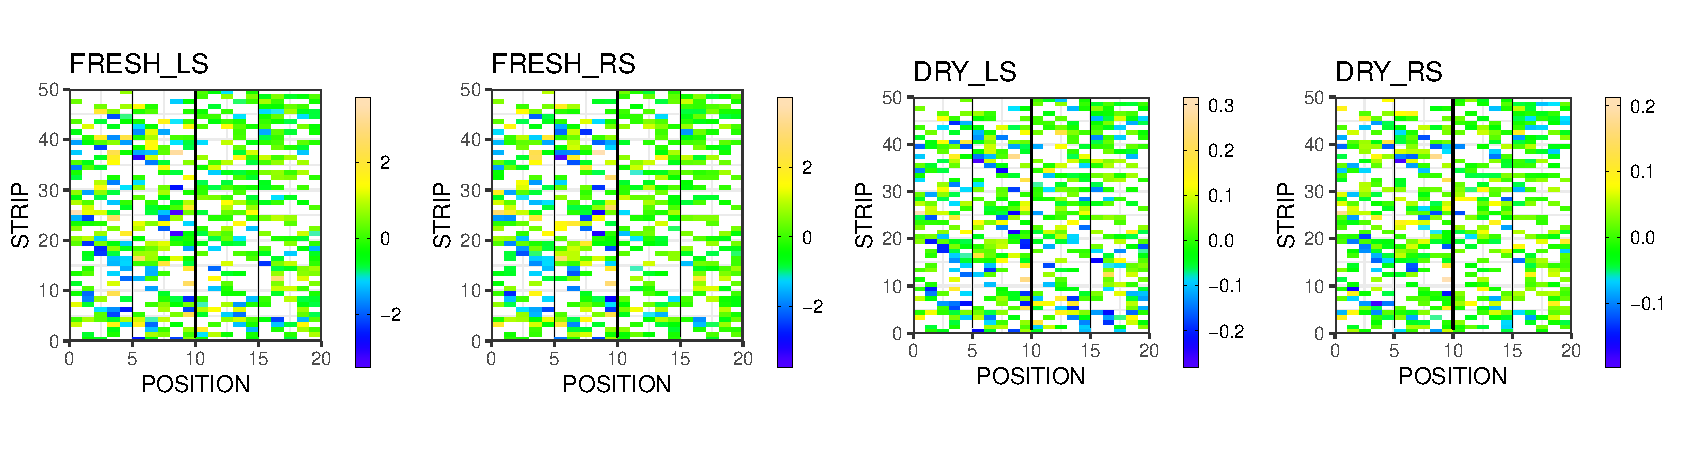
\includegraphics[width = \textwidth]{../../Figures/BSS_residuals_plot.pdf}
		\caption{Residuals' spatial plot}
	\end{subfigure}
	\caption{Raw data, fitted spatial trend and residuals' plot for each variable.}
	\label{fig:BSS_model_results}
\end{figure}

\section{Model comparison}
\subsection{Estimation performances}
In this section we compare the two models on three different points:
\begin{itemize}
	\item The estimates of the fixed tank effect
	\item The genetic variance and the heritability
	\item The estimates of the genotypic random effects
\end{itemize}
Table \ref{tab:tank_effect_model_comparison} presents the estimates of the fixed tank effects for each model. The estimates from the BSS model are consistently lower than the ones from the SpATS model, but univariate t-tests for the difference in means using the mean value and the standard deviation, showed no significant differences\footnote{All test were performed with a significance level, $\alpha$ = 0.05.} between the estimates of the two models. Furthermore, both values are close to the weighted means by tank, obtained from the raw results (see Table \ref{tab:mean_diff_between_tanks_t_test}). Finally, the tank effect was significant for all variables and in each model, confirming the clear tank effect in this platform.\\

\begin{table}[htbp]
\rowcolors{2}{gray!25}{white}
  \centering
  \caption{Comparison of the estimated fixed tank effect for both models.}
    \begin{tabular}{llrrrr}
    \toprule
          &       & \multicolumn{1}{l}{FRESH\_LS} & \multicolumn{1}{l}{FRESH\_RS} & \multicolumn{1}{l}{DRY\_LS} & \multicolumn{1}{l}{DRY\_RS} \\
    \midrule
    Tank A & SpATS & 2,9527 & 3,7282 & 0,2164 & 0,2223 \\
           & BSS   & 2,7016 & 3,2975 & 0,2075 & 0,1959 \\
    \midrule
    Tank B & SpATS & 1,3343 & 1,1445 & 0,1622 & 0,1523 \\
          & BSS   & 1,3056 & 1,1185 & 0,1660 & 0,1606 \\
    \bottomrule
    \end{tabular}%

  \label{tab:tank_effect_model_comparison}%
\end{table}%

Table \ref{tab:geno_var_heritability} presents the genetic variability ($\sigma^2_{g}$) and the heritability ($H^2$) of all variables for both models. The SpATS model seem to be slightly more effective at estimating genotypic effects since the genetic variance is always lower than for the BSS model.\\

\begin{table}[htbp]
\rowcolors{2}{gray!25}{white}
  \centering
  \caption[Comparison of both models in term of genetic variance and heritability]{Comparison of both models in term of genetic variance ($\sigma_{g}^2$) and heritability ($H^2$) }
    \begin{tabular}{lrrrrr}
 \toprule 
  & \multicolumn{2}{c}{$\sigma_{g}^2$} & \multicolumn{2}{c}{$H^2$} \\ 
  \midrule
  & SpATS & BSS & SpATS & BSS \\
  \midrule
 \hline 
 FRESH\_LS & 0,1709 & 0,1829 & 0.72 & 0.7 \\
 FRESH\_RS & 0,2618 & 0,2644 & 0.79 & 0.75 \\ 
 DRY\_LS & 1,267E-03 & 1,339E-03 & 0.73 & 0.71 \\ 
 DRY\_RS & 6,902E-04 & 7,350E-04 & 0.83 & 0.77 \\  
 \bottomrule 
    \end{tabular}%
\label{tab:geno_var_heritability}
\end{table}%
 
The heritability used in this table is defined as the part of phenotypic variation that is due to the genotype (see section 3.4.4 of chapter 3 for more details). Just as for the variances, the heritability is higher (and therefore better) for the SpATS model than for the BSS model. This is especially true for the DRY\_RS variable, where the difference in heritability is doubled compared to the other variables. However, when we look at the estimates of the genotypic random effects between models on Figure \ref{fig:genotype_comparison_BSS_SPATS}, we see that these differences are not relevant since estimates from the two models are correlated to more than 99\%. These high correlations were expected, given the similarity between the fitted values displayed in both models (see Figure \ref{fig:spats_model_results} and Figure \ref{fig:BSS_model_results}).\\

Furthermore, the genotype orders given by the models are very similar to the ones exposed in the sorted means boxplots (Figure \ref{fig:dotplot_all_variables}), with the first two genotypes being 16 and 14. They clearly stand out in the comparison plots (Figure \ref{fig:genotype_comparison_BSS_SPATS}). The distinction of genotypes order in the DRY\_RS model is less obvious, but it is still similar to the pattern picked up in the analysis of the weighted means. Without any additional information on the genotypes, it is hard to interpret this ranking in a meaningful way.\\
 
 
 \begin{figure}
	\centering
	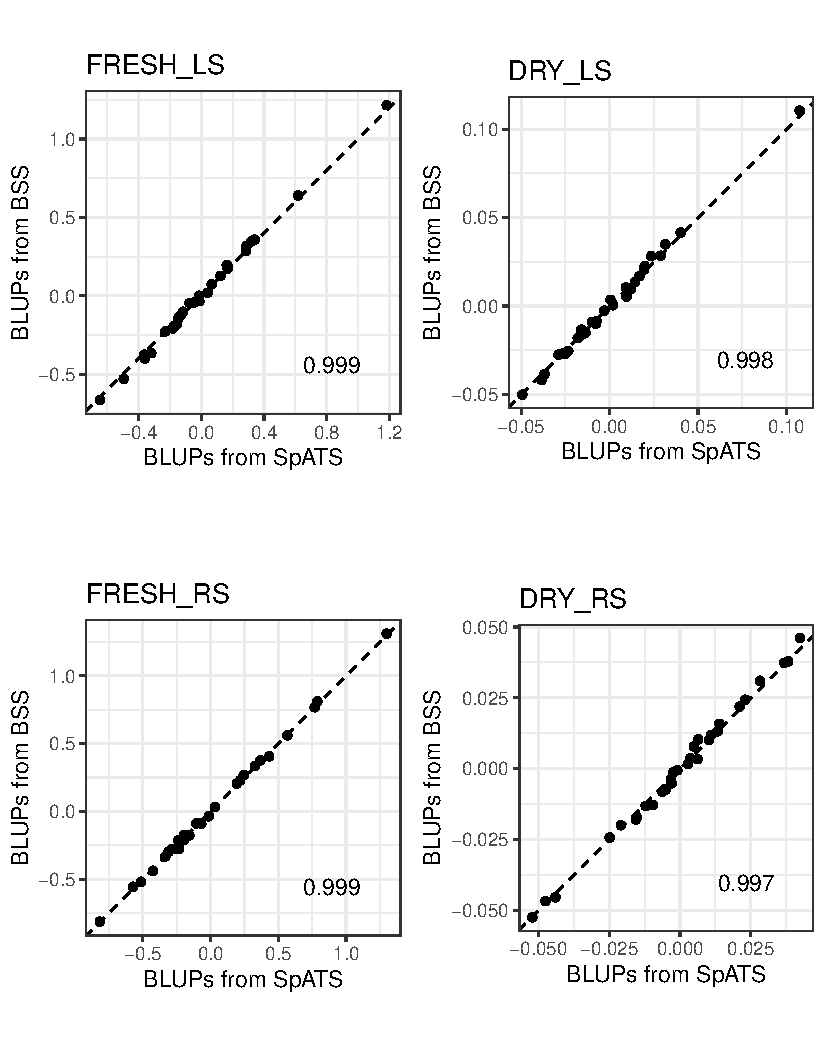
\includegraphics[width=\textwidth]{../../Figures/Genotype_Comparative_plots.pdf} 
	\caption[Comparison of the genotype BLUPs from the SpATS model and the BSS model]{Comparison of the genotype BLUPs from the SpATS model and the BSS model, with the Pearson correlation (bottom right corner of each panel).}
	\label{fig:genotype_comparison_BSS_SPATS}
\end{figure}

In conclusion of this comparison, both models yield very similar results in terms of fitted values. This similarity is reflected in the estimated tank effects and in the genotypic variances. However those variances were sligthly lower for the SpATS model, but that did not impact the estimates of the genotypic effects.\\

\subsection{Parametrization}

In terms of parametrization, both models are similar in their formulation of the spatial model as a mixed model. They include the same fixed effects and the same basic random effects (such as genotype). The major difference between both models is in the way they account for extra spatial variation. The BSS model fits a variogram over spatially dependant and independent residuals,using either an auto-regressive process or a linear variance structure, whereas the SpATS model uses tensor product of P-splines.\\

A main disadvantage of the BSS model is that it uses the basic mixed model to account for global trends and the fitted variogram to account for the local trends. This distinction between global and local can lead to variance underestimation issues \parencite{zimmerman_random_1991} or local trends overestimation issues \parencite{gumpertz1991raleigh}, when the global trends are not well accounted for. Conversely, SpATS models all the field trends (both global and local) in a single continuous process, thus avoiding the distinction between global and local trends.\\

Another disadvantage is the process that the BSS is modelling. It contains both the random and the spatially correlated data as a single term. Theoretically, only the spatially dependent data should be captured by the model and the remaining variation should be random. However, several authors showed that a part of the random error is often modelled as spatially correlated data \parencite{cullis_spatial_1998,piepho_problems_2015}. This is especially true for models with high auto-correlation values like ours, where there is a possibility of confounding between rows and columns and spatial covariance structure. Nevertheless, these issues are dampened when using a linear variance structure, as we did with the dry weights.\\

However, the weakness of the SpATS models resides in its covariance structure. The BSS model allows for more diverse way of modelling the spatial covariance structure, even using non-linear terms, whereas the SpATS model only has a linear structure. Since no studies have been conducted on this matter, it is hard to estimate how much it affects spatial modelling in field trials \parencite{velazco_modelling_2017}.
 